\chapter{الحفز}\label{ch:g12:catalysis}

تبقى قارورة من \omterm{def:g2:mixing-and-dissolving:dissolve}{محلول} بيروكسيد الهيدروجين في خزانة الحمّام
شهورًا دون تغيّر. فإذا صُبّ على ركبة مسلوخة أزبد فورًا:
فشيء ما في الدم يجعله يتفكك في ثوانٍ إلى ماء
وأكسجين. وذلك الشيء لا يُستهلك، ولا يظهر في
معادلة التفاعل. إنه حفّاز. والحفّازات تجعل معظم
الصناعة الكيميائية ممكنة، وتنقّي عوادم السيارات، وتدير كل
تفاعل من تفاعلات الحياة.

\begin{recall}
سرعة التفاعل والعوامل الحركية التي تغيّرها
(\cref{ch:g12:reaction-rates}). والآلية سلسلة من الخطوات
الأولية، مرورًا بوسائط (\cref{ch:g12:curly-arrows}).
\end{recall}

\section{ما الحفّاز}

\begin{definition}[الحفّاز، الحفز]\label{def:g12:catalysis:catalyst}
\emph{الحفّاز}\index{حفاز} \omterm{def:g6:pure-substances-and-mixtures:species}{نوع كيميائي} يجعل التفاعل
أسرع دون أن يُستهلك: فهو يشارك في الآلية لكنه يُعاد،
دون تغيّر، في النهاية، ولا يظهر في المعادلة
الإجمالية. وتسريع التفاعل بحفّاز هو
\emph{الحفز}\index{حفز}.
\end{definition}

\begin{proposition}[الحفّاز يغيّر الطريق لا الوجهة]\label{prop:g12:catalysis:path}
يفتح \omterm{def:g12:catalysis:catalyst}{الحفّاز} آلية مختلفة، حواجزها الطاقية أدنى
من حاجز التفاعل غير المحفَّز، فتنجح نسبة أكبر من اللقاءات
بين الجسيمات. ولا يغيّر \omterm{def:g7:chemical-reactions:reactant}{النواتج} المتكوّنة، ولا
\omterm{def:g10:reaction-progress-table:system}{الحالة النهائية} المبلوغة؛ بل يبلغها أسرع فحسب.
\end{proposition}

\begin{proof}
نقبله: فالمخطط الطاقي يُدرس في مجلد السنة الأولى. أما أن \omterm{def:g10:reaction-progress-table:system}{الحالة
النهائية} لا تتغير فيأتي من أن \omterm{def:g12:catalysis:catalyst}{الحفّاز} يُعاد: فالتفاعل
الإجمالي، بمتفاعلاته ونواتجه، هو نفسه.
\end{proof}

\begin{omfigure}
\begin{minipage}{0.49\linewidth}
\begin{tikzpicture}
\begin{axis}[width=\linewidth, height=5.4cm, xmin=0, xmax=1, ymin=-60,
    ymax=110, xtick=\empty, ytick=\empty, axis lines*=left,
    xlabel={تقدّم التفاعل}, ylabel={الطاقة},
    label style={font=\small}, legend style={font=\scriptsize,
    at={(0.02,0.99)}, anchor=north west, draw=none}, legend cell align=left]
  \addplot[very thick, omDef] table[x=s, y=Eu] {figdata/out/grade-12-catalysis-a.dat};
  \addplot[very thick, omProp] table[x=s, y=Ec] {figdata/out/grade-12-catalysis-a.dat};
  \legend{{دون حفّاز}, {مع حفّاز}}
  \node[font=\scriptsize, anchor=north west] at (axis cs:0.02,-4) {المتفاعلات};
  \node[font=\scriptsize, anchor=south east] at (axis cs:0.99,-36) {النواتج};
\end{axis}
\end{tikzpicture}
\end{minipage}\hfill
\begin{minipage}{0.49\linewidth}
\begin{tikzpicture}
\begin{axis}[width=\linewidth, height=5.4cm, xmin=0, xmax=60, ymin=0,
    ymax=80, xlabel={\babelsublr{$t$ (\si{min})}}, ylabel={\foreignlanguage{arabic}{\ce{O2} المنطلق \babelsublr{(\si{mL})}}},
    axis lines*=left, ymajorgrids, grid style={gray!20},
    tick label style={font=\scriptsize}, label style={font=\small},
    legend style={font=\scriptsize, at={(0.98,0.03)}, anchor=south east,
    draw=none}, legend cell align=left]
  \addplot[very thick, omDef] table[x=t, y=Vu] {figdata/out/grade-12-catalysis-b.dat};
  \addplot[very thick, omProp] table[x=t, y=Vc] {figdata/out/grade-12-catalysis-b.dat};
  \legend{{دون حفّاز}, {مع حفّاز}}
\end{axis}
\end{tikzpicture}
\end{minipage}

{\small يسارًا: الطاقة على امتداد التفاعل؛ يمر الطريق المحفَّز
بوسيط وحاجزين أدنى. يمينًا: الأكسجين المنطلق من
\omterm{def:g2:mixing-and-dissolving:dissolve}{محلول} بيروكسيد الهيدروجين؛ يسرّع \omterm{def:g12:catalysis:catalyst}{الحفّاز} التفاعل، لكن
الحجم النهائي هو نفسه. (منحنيات نموذجية.)}
\end{omfigure}

\section{الحفز المتجانس}

\begin{definition}[الحفز المتجانس وغير المتجانس]\label{def:g12:catalysis:homogeneous}
يكون \omterm{def:g12:catalysis:catalyst}{الحفز} \emph{حفزًا متجانسًا}\index{حفز متجانس}
حين يكون \omterm{def:g12:catalysis:catalyst}{الحفّاز} في طور \omterm{def:g7:chemical-reactions:reactant}{المتفاعلات} نفسه (مثلًا
مذابًا معها)، و\emph{حفزًا غير متجانس}\index{حفز غير متجانس}
حين يكون في طور آخر، غالبًا صلب تبلغ المتفاعلاتُ
سطحَه من غاز أو سائل.
\end{definition}

\begin{example}[أيونات اليوديد وبيروكسيد الهيدروجين]\label{ex:g12:catalysis:iodide}
يتفكك بيروكسيد الهيدروجين وحده ببطء شديد:
\ce{2H2O2 -> 2H2O + O2}. فإذا أذيب فيه قليل من يوديد البوتاسيوم،
أزبد فورًا. \omterm{def:g9:ions:ion}{فأيون} اليوديد يفتح طريقًا من خطوتين:
\[
  \ce{H2O2 + I- -> H2O + IO-}, \qquad
  \ce{H2O2 + IO- -> H2O + O2 + I-} .
\]
وبجمع الخطوتين نعود إلى \ce{2H2O2 -> 2H2O + O2}: \omterm{def:g9:ions:ion}{فأيون} اليوديد،
المستهلك في الخطوة الأولى والمُعاد في الثانية، هو \omterm{def:g12:catalysis:catalyst}{الحفّاز}؛
\omterm{def:g9:ions:ion}{والأيون} \ce{IO-} وسيط.
\end{example}


\begin{example}[أيونات الحديد (III)]\label{ex:g12:catalysis:iron}
تحفّز \omterm{def:g9:ions:ion}{أيونات} الحديد (III) أيضًا هذا التفكك، عبر المزدوجة
$\ce{Fe^{3+}}/\ce{Fe^{2+}}$ (\cref{ch:g11:redox}): فهي تؤكسد أولًا
بيروكسيد الهيدروجين، \ce{2Fe^{3+} + H2O2 -> 2Fe^{2+} + O2 + 2H+}، ثم تُؤكسد
\omterm{def:g9:ions:ion}{أيونات} الحديد (II) المتكوّنة من جديد بمزيد من بيروكسيد الهيدروجين،
\ce{2Fe^{2+} + H2O2 + 2H+ -> 2Fe^{3+} + 2H2O}. فيصير اللون البرتقالي الباهت
\omterm{def:g2:mixing-and-dissolving:dissolve}{للمحلول} مخضرًّا بينما ينطلق الغاز، ثم يعود
حين يُستهلك بيروكسيد الهيدروجين: دليل على أن \omterm{def:g12:catalysis:catalyst}{الحفّاز} يشارك
ثم يتجدد.
\end{example}

\section{الحفز غير المتجانس}

كثير من الحفّازات الصناعية أجسام صلبة: \omterm{def:g9:periodic-table-first-look:metal}{فلزات} كالبلاتين والبلاديوم
والنيكل والحديد، أو أكاسيد. ويجري التفاعل على سطحها،
في ثلاث مراحل: تُمسك \omterm{def:g7:atoms-and-molecules:molecule}{جزيئات} \omterm{def:g7:chemical-reactions:reactant}{المتفاعلات} على السطح
(تُمتزّ)، حيث تضعف روابطها؛ ثم تتفاعل هناك؛ ثم تغادر
\omterm{def:g7:chemical-reactions:reactant}{النواتج} السطح، فيتحرر \omterm{def:g7:atoms-and-molecules:molecule}{لجزيئات} جديدة. لذلك يُصنع \omterm{def:g12:catalysis:catalyst}{الحفّاز}
بأكبر سطح ممكن: مسحوقًا ناعمًا، أو طبقة
رقيقة على حامل مسامي.

\begin{omfigure}
\begin{tikzpicture}[font=\small]
  \foreach \x in {0,4.2,8.4} {
    \fill[black!25] (\x,0) rectangle (\x+3.4,0.35);
    \foreach \i in {0,1,2,3,4,5,6,7} \shade[ball color=black!35] (\x+0.21+\i*0.425,0.35) circle (0.2);
  }
  % 1. adsorption
  \node[aH, minimum size=3.2mm] at (0.9,0.75) {};
  \node[aH, minimum size=3.2mm] at (1.3,0.75) {};
  \node[aH, minimum size=3.2mm] (h1) at (2.2,1.8) {};
  \node[aH, minimum size=3.2mm] (h2) at (2.6,1.8) {};
  \draw[bond, line width=1.2pt] (h1.east) -- (h2.west);
  \draw[->, omProp, thick] (2.4,1.55) -- (2.0,1.0);
  \node[anchor=north, align=center] at (1.7,-0.1) {\foreignlanguage{arabic}{\babelsublr{1.} امتزاز:}\\ \foreignlanguage{arabic}{تنكسر الرابطة \ce{H-H}}};
  % 2. reaction on the surface
  \node[aC] (c1) at (5.5,1.05) {}; \node[aC] (c2) at (6.2,1.05) {};
  \draw[bond, line width=1.4pt] (c1) -- (c2);
  \node[aH, minimum size=3.2mm] at (5.3,0.75) {};
  \node[aH, minimum size=3.2mm] at (6.6,0.75) {};
  \node[anchor=north, align=center] at (5.9,-0.1) {\foreignlanguage{arabic}{\babelsublr{2.} تنضم ذرتا \babelsublr{H}}\\ إلى الجزيء الممتزّ};
  % 3. desorption
  \node[aC] (c3) at (9.6,1.8) {}; \node[aC] (c4) at (10.3,1.8) {};
  \draw[bond, line width=1.4pt] (c3) -- (c4);
  \foreach \a/\c in {150/c3,210/c3,90/c3,30/c4,-30/c4,90/c4}
    \node[aH, minimum size=2.8mm] at ($(\c)+(\a:0.42)$) {};
  \draw[->, omProp, thick] (11.0,1.2) -- (11.0,2.2);
  \node[anchor=north, align=center] at (10.1,-0.1) {\foreignlanguage{arabic}{\babelsublr{3.} يغادر الناتج}\\ السطح};
\end{tikzpicture}

{\small إضافة الهيدروجين إلى الإيثين على سطح \omterm{def:g9:periodic-table-first-look:metal}{فلز}: امتزاز، ثم
تفاعل، ثم مغادرة السطح. ويُعاد \omterm{def:g9:periodic-table-first-look:metal}{الفلز} دون تغيّر.}
\end{omfigure}

\begin{example}[المحوّل الحفّاز]\label{ex:g12:catalysis:converter}
يحوي عادم محرك البنزين أحادي أكسيد الكربون وأحادي أكسيد
النيتروجين، وكلاهما سام، ووقودًا لم يحترق. وفي المحوّل \omterm{def:g12:catalysis:catalyst}{الحفّاز}،
وهو قرص خزفي على هيئة خلية نحل مغطى بالبلاتين والروديوم، تتفاعل على
سطح \omterm{def:g9:periodic-table-first-look:metal}{الفلز}:
\[
  \ce{2CO + 2NO -> 2CO2 + N2} ,
\]
وتحترق الهيدروكربونات إلى ثنائي أكسيد الكربون وماء. وتعبر الغازات
المحوّل في جزء من الثانية، وهي مدة أقصر من أن يجري فيها أي تفاعل
دون حفّاز.
\end{example}

\begin{omfigure}
\begin{tikzpicture}[font=\small]
  \fill[black!12, draw=black!60, rounded corners=6pt] (0,0) rectangle (6,2.4);
  \foreach \x in {0.3,0.6,0.9,1.2,1.5,1.8,2.1,2.4,2.7,3.0,3.3,3.6,3.9,4.2,4.5,4.8,5.1,5.4,5.7} \draw[black!35] (\x,0.2) -- (\x,2.2);
  \foreach \y in {0.5,0.9,1.3,1.7,2.1} \draw[black!35] (0.2,\y) -- (5.8,\y);
  \fill[black!40] (-1.4,0.9) rectangle (0,1.5);
  \fill[black!40] (6,0.9) rectangle (7.4,1.5);
  \draw[->, very thick, omThm] (-2.6,1.2) -- (-1.5,1.2);
  \node[anchor=east, align=right, omThm] at (-2.7,1.2) {\foreignlanguage{arabic}{\ce{CO}، \ce{NO}،}\\ هيدروكربونات};
  \draw[->, very thick, omMeth] (7.5,1.2) -- (8.6,1.2);
  \node[anchor=west, align=left, omMeth] at (8.7,1.2) {\foreignlanguage{arabic}{\ce{CO2}، \ce{N2}،}\\ \ce{H2O}};
  \node[align=center, fill=white, inner sep=2pt] at (3,1.2) {خلية نحل خزفية\\ \foreignlanguage{arabic}{مغطاة بفلزي \babelsublr{Pt} و\babelsublr{Rh}}};
\end{tikzpicture}

{\small محوّل حفّاز في مقطع طولي: آلاف القنوات الرفيعة
تمنح غازات العادم سطحًا هائلًا مغطى \omterm{def:g9:periodic-table-first-look:metal}{بالفلز}.}
\end{omfigure}

\begin{omfigure}
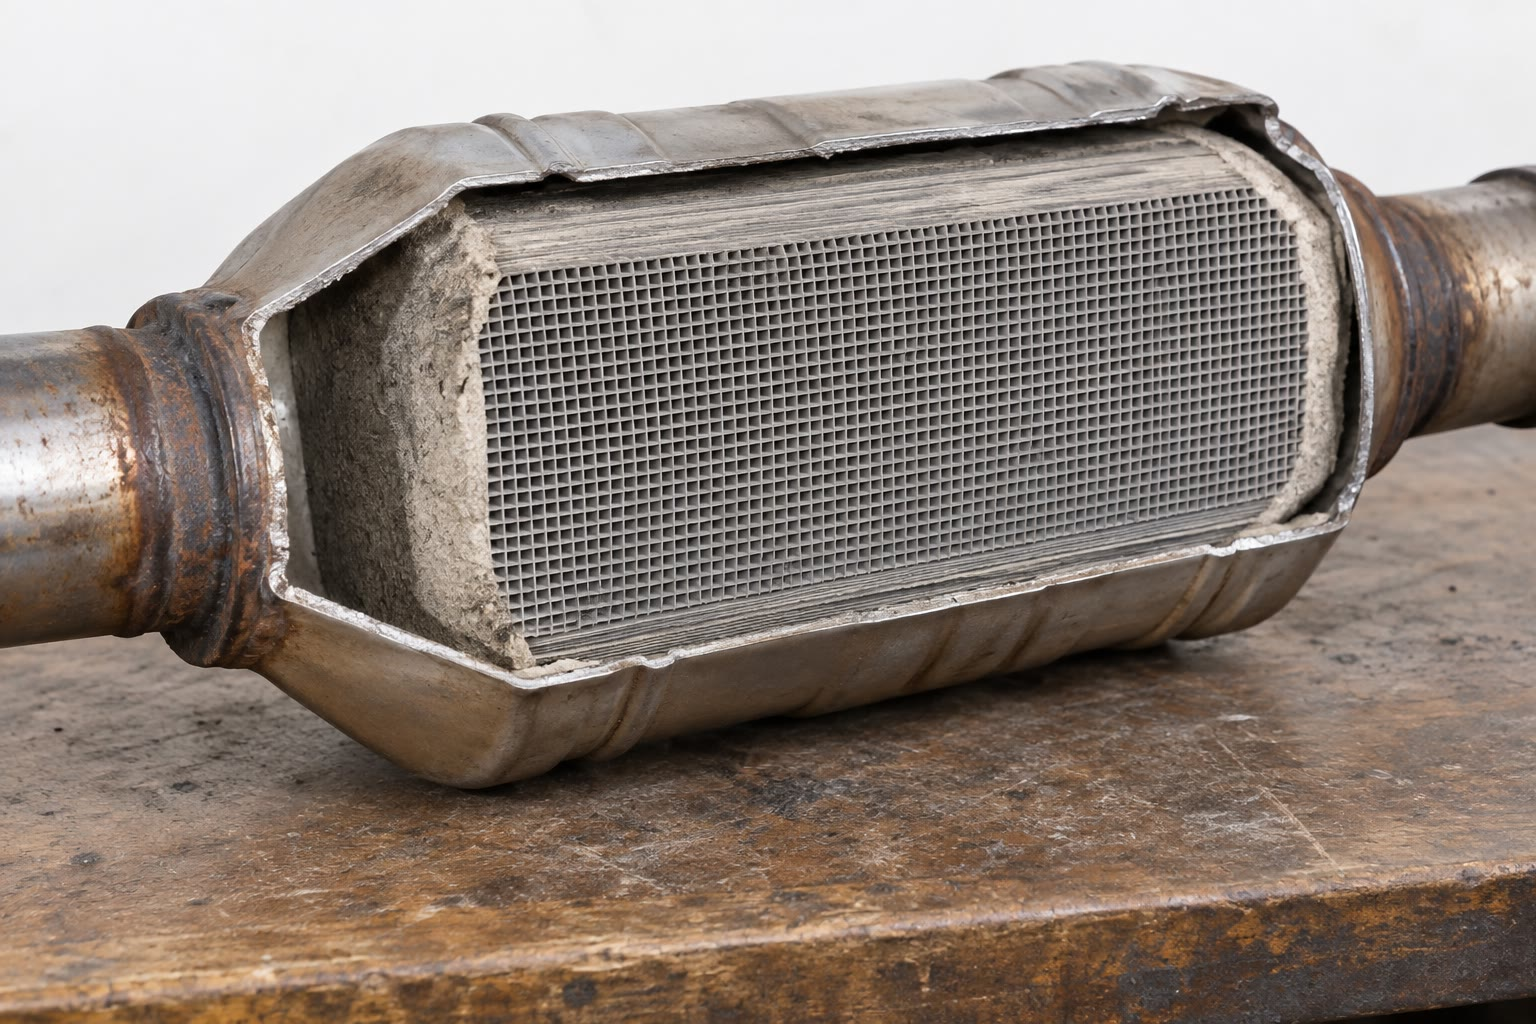
\includegraphics[width=0.45\linewidth]{images/book1/ai/g12-catalytic-converter.jpg}

{\small محوّل حفّاز مفتوح: قلبه على هيئة خلية نحل.}
\end{omfigure}

\begin{history}[هابر وبوش والأمونيا]
% ledger: haber:T, haber:p, nh3:world-2024
في مطلع القرن العشرين اكتشف الكيميائي فريتز هابر
كيف يُجمع نيتروجين \omterm{def:g4:air-a-mixture-of-gases:air}{الهواء} بالهيدروجين،
\ce{N2 + 3H2 -> 2NH3}، على حفّاز أساسه الحديد، وحوّل المهندس كارل
بوش ذلك إلى عملية صناعية. وما زالت تجري اليوم عند 400
إلى \qty{500}{\celsius} وتحت 150 إلى \qty{250}{atm}. وفي سنة 2024 صنع العالم
أمونيا تحوي نحو 150 مليون طن من النيتروجين، معظمها
للأسمدة: فجزء كبير من النيتروجين الموجود في الغذاء الذي نأكله مرّ
بحفّاز من هذا النوع.
\end{history}

\section{الإنزيمات}

\begin{definition}[الإنزيم]\label{def:g12:catalysis:enzyme}
\emph{الإنزيم}\index{إنزيم} بروتين يصنعه كائن حي
ويحفّز تفاعلًا واحدًا من تفاعلات كيميائه. والإنزيمات فعّالة جدًا
وانتقائية جدًا: فكل منها لا يناسب إلا \omterm{def:g7:atoms-and-molecules:molecule}{جزيئات} قليلة، وتعمل على أفضل وجه في
مجال ضيق من درجة الحرارة والحموضة.
\end{definition}

\begin{example}[الكاتالاز]\label{ex:g12:catalysis:catalase}
يتكوّن بيروكسيد الهيدروجين في الخلايا ناتجًا ثانويًا، وهو ضار
بها. \omterm{def:g12:catalysis:enzyme}{وإنزيم} الكاتالاز، الموجود في الدم والكبد وكثير من الأنسجة
النباتية، يفككه إلى ماء وأكسجين بسرعة هائلة: وذلك هو
الزبد على الركبة المسلوخة، أو على شريحة بطاطس نيئة. أما البطاطس المسلوقة
فلا تعطي زبدًا: فقد أتلف التسخين شكل \omterm{def:g12:catalysis:enzyme}{الإنزيم}.
\end{example}

\begin{omfigure}
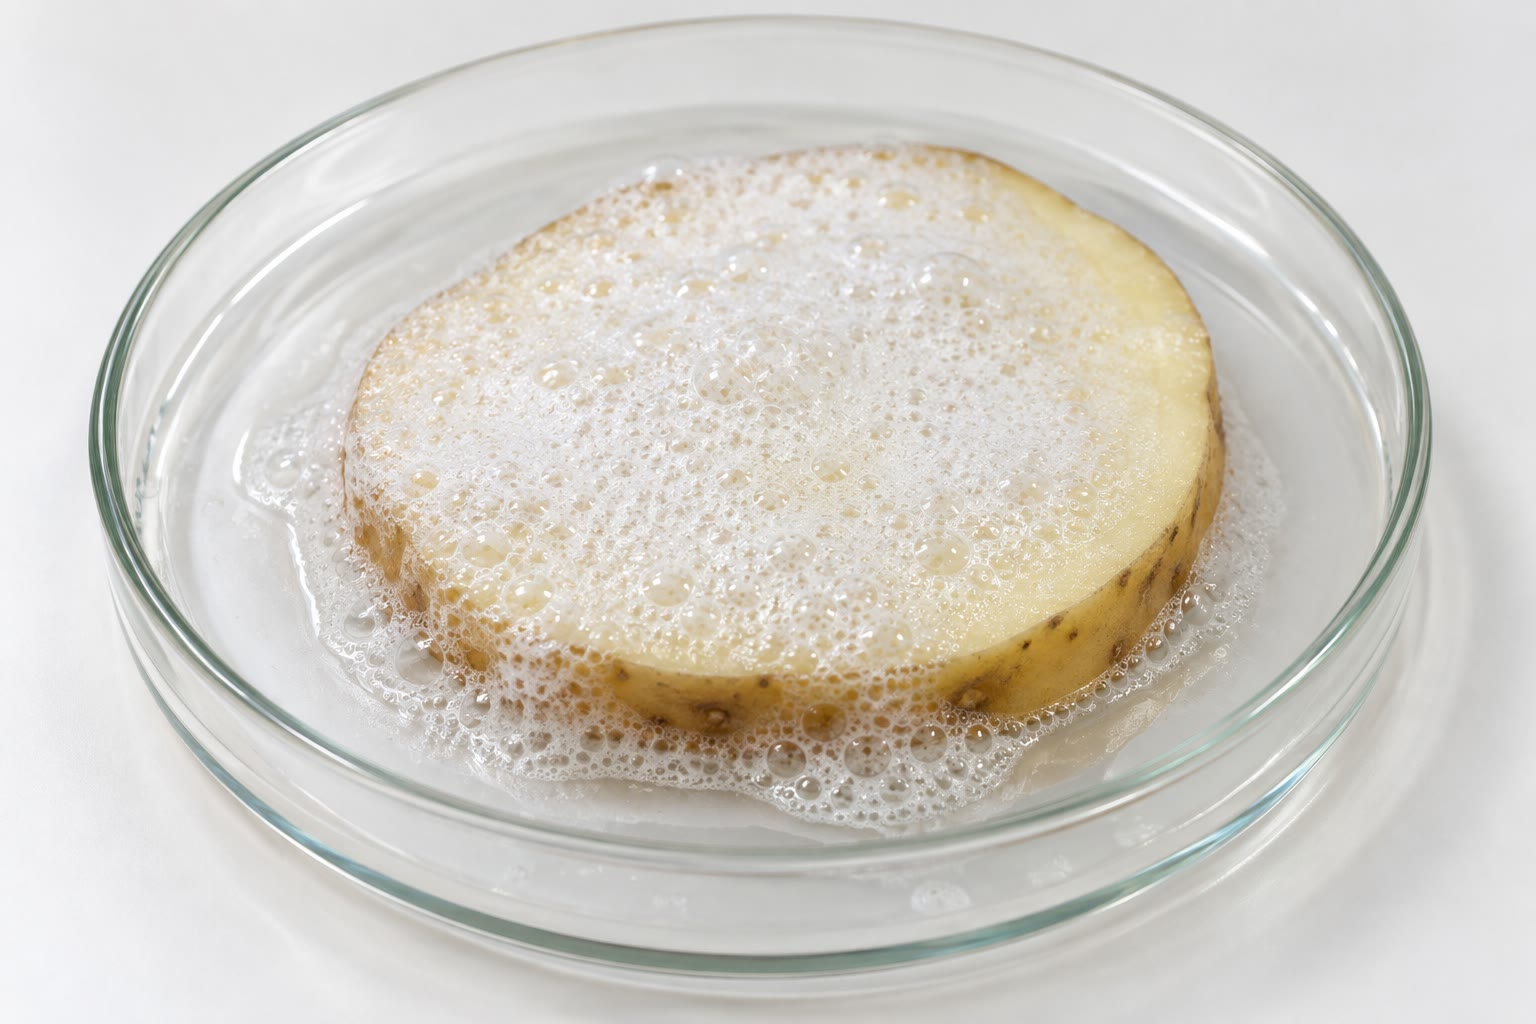
\includegraphics[width=0.45\linewidth]{images/book1/ai/g12-potato-peroxide.jpg}

{\small بيروكسيد الهيدروجين على شريحة بطاطس نيئة: الكاتالاز يعمل.}
\end{omfigure}

\section{الانتقائية}

\begin{definition}[الحفّاز الانتقائي]\label{def:g12:catalysis:selective}
حين تستطيع \omterm{def:g7:chemical-reactions:reactant}{المتفاعلات} نفسها أن تعطي عدة تفاعلات، فإن \emph{الحفّاز
الانتقائي}\index{حفاز انتقائي} يسرّع أحدها أكثر بكثير من
غيره، فيحدد بذلك \omterm{def:g7:chemical-reactions:reactant}{النواتج} التي تتكوّن.
\end{definition}

\begin{example}[مصيران للإيثانول]\label{ex:g12:catalysis:ethanol}
بخار الإيثانول الساخن المار فوق الألومينا يفقد الماء ويعطي الإيثين،
\ce{C2H5OH -> C2H4 + H2O} (حذف)؛ والمار فوق النحاس الساخن
يفقد الهيدروجين ويعطي الإيثانال، \ce{C2H5OH -> CH3CHO + H2}. \omterm{def:g7:chemical-reactions:reactant}{المتفاعل}
نفسه، وحفّازان، وناتجان.
\end{example}

\begin{remark}[الصناعة والحياة تقومان على الحفّازات]\label{rem:g12:catalysis:everywhere}
معظم منتجات الصناعة الكيميائية، من \omterm{def:g4:what-a-fire-needs:fuel}{الوقود} إلى \omterm{def:g8:plastics:plastic}{البلاستيك}
والأسمدة، تُصنع بحفّازات؛ وإيجاد حفّاز أنشط أو أكثر
انتقائية يوفّر الطاقة ويقلل النفايات. وكل تفاعل في الخلية
الحية يحفّزه \omterm{def:g12:catalysis:enzyme}{إنزيم}.
\end{remark}

\begin{safety}{\ghs[0.82cm]{GHS03}\ghs[0.82cm]{GHS05}\ghs[0.82cm]{GHS07}}
% ledger: ghs:H2O2
بيروكسيد الهيدروجين المركّز \omterm{def:g11:redox:oxidant}{مؤكسد} قوي قد يغذي حريقًا،
ويحرق الجلد والعينين، وهو ضار إذا ابتُلع. ومحاليله المخففة
في المختبر تحتاج هي أيضًا إلى نظارتين واقيتين وقفازين؛ وتفككه
يطلق الأكسجين، فلا يُجرى أبدًا في وعاء مغلق.
\end{safety}

\section{تمارين}


\begin{exercise}[$\star$]\label{exo:g12:catalysis:1}
في تفكك بيروكسيد الهيدروجين المحفَّز \omterm{def:g9:ions:ion}{بأيونات} اليوديد، أي
الأنواع متفاعلات، وأيها نواتج، وأيها \omterm{def:g12:catalysis:catalyst}{الحفّاز}، وأيها
وسيط؟
\end{exercise}

\begin{exercise}[$\star$]\label{exo:g12:catalysis:2}
\omterm{def:g12:catalysis:homogeneous}{حفز متجانس} أم غير متجانس: \omterm{def:g9:ions:ion}{أيونات} اليوديد في \omterm{def:g2:mixing-and-dissolving:dissolve}{محلول} بيروكسيد
الهيدروجين؛ البلاتين في محوّل حفّاز؛ الحديد في تصنيع
الأمونيا؛ \omterm{def:g9:ions:ion}{أيونات} الحديد (III) في \omterm{def:g2:mixing-and-dissolving:dissolve}{محلول} بيروكسيد الهيدروجين؟
\end{exercise}

\begin{exercise}[$\star$]\label{exo:g12:catalysis:3}
في المخططين الطاقيين، أي الطريقين حاجزه أعلى؟ وهل الطاقتان
الابتدائية والنهائية هما نفسهما في الطريقين؟ وماذا يعني ذلك
بالنسبة إلى \omterm{def:g7:chemical-reactions:reactant}{النواتج}؟
\end{exercise}

\begin{exercise}[$\star$]\label{exo:g12:catalysis:4}
لماذا لا يظهر \omterm{def:g12:catalysis:catalyst}{الحفّاز} في المعادلة الإجمالية للتفاعل؟
\end{exercise}

\begin{exercise}[$\star$]\label{exo:g12:catalysis:5}
لماذا تُستعمل الحفّازات الصلبة في الصناعة مساحيق ناعمة أو طبقات
رقيقة على حوامل مسامية؟
\end{exercise}

\begin{exercise}[$\star\star$]\label{exo:g12:catalysis:6}
اجمع خطوتي تفكك بيروكسيد الهيدروجين المحفَّز بالحديد (III)،
وبيّن أن \omterm{def:g9:ions:ion}{أيونات} الحديد \omterm{def:g9:ions:ion}{وأيونات} الهيدروجين تُحذف من الطرفين.
\end{exercise}

\begin{exercise}[$\star\star$]\label{exo:g12:catalysis:7}
اقرأ منحنيي الأكسجين المنطلق. كم من الوقت تستغرق كل تجربة
لإطلاق نصف الحجم النهائي؟ وبأي عامل يقصّر
\omterm{def:g12:catalysis:catalyst}{الحفّاز} هذه المدة؟
\end{exercise}

\begin{exercise}[$\star\star$]\label{exo:g12:catalysis:8}
لا يُستعمل البنزين المحتوي على الرصاص في السيارات المزودة بمحوّل حفّاز: إذ
يترسب الرصاص على البلاتين ويبقى عليه. اشرح لماذا يُتلف ذلك
المحوّل، مع أن البلاتين لا يُستهلك في التفاعل العادي.
\end{exercise}

\begin{exercise}[$\star\star$]\label{exo:g12:catalysis:9}
يقيس طالب الزبد الذي تنتجه شرائح البطاطس في بيروكسيد
الهيدروجين عند 10 و25 و37 و60 و\qty{80}{\celsius}: فيزداد الزبد حتى
نحو \qty{37}{\celsius}، ثم يقل، ويكاد يختفي عند
\qty{80}{\celsius}. فسّر جزأي المنحنى.
\end{exercise}

\begin{exercise}[$\star\star$]\label{exo:g12:catalysis:10}
اكتب معادلة التفاعل في المحوّل \omterm{def:g12:catalysis:catalyst}{الحفّاز} بين
أحادي أكسيد الكربون وأحادي أكسيد النيتروجين، وتحقق من أنها موزونة.
ولماذا يُزال الملوِّثان معًا؟
\end{exercise}

\begin{exercise}[$\star\star$]\label{exo:g12:catalysis:11}
يطلق \qty{10.0}{mL} من \omterm{def:g2:mixing-and-dissolving:dissolve}{محلول} بيروكسيد الهيدروجين \qty{72}{mL} من
الأكسجين عند \qty{20}{\celsius} حين يتفكك كليًا. احسب
كمية الأكسجين ($V_m = \qty{24.1}{L/mol}$)، ثم تركيز
\omterm{def:g2:mixing-and-dissolving:dissolve}{المحلول} من بيروكسيد الهيدروجين.
\end{exercise}

\begin{exercise}[$\star\star\star$]\label{exo:g12:catalysis:12}
يعطي بخار الإيثانول المار فوق الألومينا الإيثين؛ وفوق النحاس يعطي
الإيثانال. اكتب المعادلتين، وأعطِ فئة الأولى،
واشرح ما \omterm{def:g12:catalysis:selective}{الحفّاز الانتقائي}.
\end{exercise}

\begin{exercise}[$\star\star\star$]\label{exo:g12:catalysis:13}
يجعل حفّاز تفاعلًا أسرع بعشر مرات. فيدّعي طالب أنه يعطي أيضًا
عشرة أضعاف \omterm{def:g7:chemical-reactions:reactant}{الناتج}. صحّح الادعاء، مستعينًا بمنحنيي
الأكسجين المنطلق.
\end{exercise}

\begin{exercise}[$\star\star\star$]\label{exo:g12:catalysis:14}
يفكك \omterm{def:g7:atoms-and-molecules:molecule}{جزيء} من الكاتالاز بضعة ملايين من \omterm{def:g7:atoms-and-molecules:molecule}{جزيئات}
بيروكسيد الهيدروجين في الثانية. فإذا أخذنا $\num{5e6}$ في الثانية، فكم من الوقت
يستغرق \omterm{def:g7:atoms-and-molecules:molecule}{جزيء} \omterm{def:g12:catalysis:enzyme}{إنزيم} واحد لتفكيك \omterm{def:g10:the-mole:amount}{مول} واحد من بيروكسيد الهيدروجين؟
وكم جزيئًا من \omterm{def:g12:catalysis:enzyme}{الإنزيم} يلزم لتفكيكه في ثانية واحدة؟ (حساب لرتب
المقادير؛ والسرعة معطى من معطيات التمرين.)
\end{exercise}

\begin{exercise}[$\star\star\star$]\label{exo:g12:catalysis:15}
% ledger: nh3:world-2024
صنع العالم نحو 150 مليون طن من النيتروجين في الأمونيا سنة 2024.
فما كتلة الأمونيا الموافقة؟ وما كمية ثنائي النيتروجين التي جُمعت؟
\end{exercise}

\section{مسألة: بيروكسيد الحلّاق}

\begin{problem}[{مسألة نهاية الأسبوع --- ما تركيز بيروكسيد الهيدروجين
«20 حجمًا»؟}]
\label{pb:g12:catalysis:1}
% ledger: const:Vm1, ghs:H2O2, aw:H, aw:O
يستعمل الحلّاقون محاليل بيروكسيد الهيدروجين موسومة «بالأحجام»: \omterm{def:g2:mixing-and-dissolving:dissolve}{فالمحلول}
«20 حجمًا» هو الذي يطلق \qty{1}{L} منه \qty{20}{L}
من الأكسجين حين يتفكك كليًا، والغاز مقيس عند
\qty{0}{\celsius} وتحت الضغط الجوي العادي، حيث يشغل \omterm{def:g10:the-mole:amount}{المول} الواحد من الغاز
\qty{22.4}{L}.

\medskip
\noindent\textbf{الجزء الأول --- التفكك.}
\begin{enumerate}
  \item اكتب معادلة تفكك بيروكسيد الهيدروجين.
  \item أهذا التفكك \omterm{def:g11:redox:reaction}{تفاعل أكسدة واختزال}؟ جد \omterm{def:g11:redox:oxidant}{المؤكسد}
        \omterm{def:g11:redox:oxidant}{والمختزل} (فبيروكسيد الهيدروجين هو الاثنان معًا).
  \item لماذا تبقى القارورة صالحة شهورًا، مع أن التفاعل
        ممكن؟
\end{enumerate}

\medskip
\noindent\textbf{الجزء الثاني --- ما معنى «20 حجمًا».}
\begin{enumerate}[resume]
  \item ما كمية الأكسجين التي يطلقها \qty{1}{L} من \omterm{def:g2:mixing-and-dissolving:dissolve}{المحلول}؟
  \item استنتج كمية بيروكسيد الهيدروجين في \qty{1}{L}.
  \item أعطِ \omterm{def:g10:concentration-and-dilution:molar-concentration}{التركيز المولي}.
  \item احسب \omterm{def:g10:the-mole:molar-mass}{الكتلة المولية} لبيروكسيد الهيدروجين \omterm{def:g10:concentration-and-dilution:mass-concentration}{والتركيز
        الكتلي}.
  \item ماذا تعني «10 أحجام» \omterm{def:g10:the-mole:amount}{بالمول} في اللتر؟
\end{enumerate}

\medskip
\noindent\textbf{الجزء الثالث --- حفّازان.}
\begin{enumerate}[resume]
  \item تضاف إلى عيّنة قطرة دم (كاتالاز)، وإلى أخرى بضع قطرات من كلوريد الحديد (III).
        فأي نوع من \omterm{def:g12:catalysis:catalyst}{الحفز} في كل حالة؟
  \item اكتب خطوتي \omterm{def:g12:catalysis:catalyst}{الحفز} بالحديد (III) وتحقق من أن
        مجموعهما هو التفكك.
  \item مستعينًا بمنحنيي الأكسجين المنطلق، صف كيف يتغير حجم
        الأكسجين مع \omterm{def:g12:catalysis:catalyst}{الحفّاز} ودونه، وما الذي يبقى
        على حاله.
  \item لماذا يتغير لون عيّنة محفَّزة بالحديد (III) خلال
        التفاعل ثم يعود في النهاية؟
  \item لماذا لا تجعل البطاطس المسلوقة \omterm{def:g2:mixing-and-dissolving:dissolve}{المحلول} يُزبد؟
\end{enumerate}

\medskip
\noindent\textbf{الجزء الرابع --- القارورة.}
\begin{enumerate}[resume]
  \item ما حجم الأكسجين، مقيسًا عند \qty{0}{\celsius}، الذي يمكن أن تطلقه
        قارورة سعتها \qty{100}{mL}؟
  \item كم يساوي هذا الحجم عند \qty{20}{\celsius} ($V_m =
        \qty{24.1}{L/mol}$)؟
  \item لماذا يجب أن تسمح سدادة هذه القارورة للغاز بالخروج ببطء؟
  \item عويرت قارورة خُزّنت مدة طويلة فوُجد أنها تحوي
        \qty{1.50}{mol/L}. فكم «حجمًا» يمثل ذلك الآن؟
  \item ما الكسر الذي تفكك من بيروكسيد الهيدروجين؟
  \item اذكر الجواب النهائي: ما \omterm{def:g10:concentration-and-dilution:molar-concentration}{التركيز المولي} \omterm{def:g2:mixing-and-dissolving:dissolve}{لمحلول} بيروكسيد
        الهيدروجين «20 حجمًا»؟
\end{enumerate}
\end{problem}
